% This is samplepaper.tex, a sample chapter demonstrating the
% LLNCS macro package for Springer Computer Science proceedings;
% Version 2.20 of 2017/10/04
%
\documentclass[runningheads]{llncs}
%
\usepackage{graphicx}
% Used for displaying a sample figure. If possible, figure files should
% be included in EPS format.
%
% If you use the hyperref package, please uncomment the following line
% to display URLs in blue roman font according to Springer's eBook style:
% \renewcommand\UrlFont{\color{blue}\rmfamily}

\begin{document}
%
\title{RBcoins: An analysis of crypto-asset backed stable coins\thanks{Supported by organization x.}}
%
%\titlerunning{Abbreviated paper title}
% If the paper title is too long for the running head, you can set
% an abbreviated paper title here
%
\author{Mehdi Salehi\inst{1} \and
Jeremy Clark\inst{1}\and
Mohammad Mannan\inst{1}}
%
\authorrunning{M. Salehi et al.}
% First names are abbreviated in the running head.
% If there are more than two authors, 'et al.' is used.
%
\institute{Concordia University \
\email{lncs@springer.com}\\
}
%
\maketitle              % typeset the header of the contribution
%
\begin{abstract}



\keywords{First keyword  \and Second keyword \and Another keyword.}
\end{abstract}


%
%
%
\section{What is RB tokens}
%%"A currency, to be perfect, should be absolutely invariable in value," said David Ricardo in 1817.
%%There is a huge debate about the charectaristics of a stable asset. One may claim that a stable asset or currency is an asset that helps its owner to have stable purchasing power. Others may claim that an stable asset should have invariable quantity.

There is a growing tendency to issue asset on top of blockchain that represents  real world assets such as shares, commodities, and currencies. 

One way to implement this kind of tokens is that a company obtains a reserve of the asset and issue tokens that represents a unit of asset. But this design needs custodianship proofs, periodic audits and also trust on the third party.

The question raised here is whether it is possible to find a solution to remove the trust on the third party?

The answer is RB token Dapp. There are two parties involving on each contract of the system. The Red token holder who need a representation of the underlying asset on the blockchain, and Black token holder who bets against the pair value of ETH and the underlying asset.

Therefore, the amount of deposited ETH on each new agreement will grow or shrink depending on the exchange rates of the underlying asset and ETH. Because a blockchain has no inherent knowledge of exchange rates, this mechanism still requires one trustworthy entity called an oracle to write the exchange rates into the blockchain (or consensus can be taken across a set of oracles).

\emph{Working Example}: Assume Alice wants to create representation of Google share (GOOGL). She sets up a DApp that can hold ETH and issue tokens. The DApp determines how much ETH is equivalent to 1.5 GOGGL, using the current exchange rates, provided to the DApp by a trusted third-party oracle, and Alice deposits this amount of ETH into the DApp. The DApp issues to Alice two tokens, Red and Black. At some future time, the holder of Red token can redeem up to equivalent value of 1 GOOGL in ETH from the deposit and the holder of the Black token gets any remaining ETH. Alice will transfer the Black token to Bob who wants to bet against ETH/GOOGL. When Alice redeems the Red token, it will be worth 1 GOOGL in ETH when the entire deposit of ETH is worth more than 1 GOOGL. If the exchange rate of ETH drops enough or the exchange rate of the GOOGL raise enough (or combinatoion of them), the entire deposit will be worth less than a 1 GOOGL—Alice will get all of the deposit, and the holder of the Black token will get nothing.

There are two risks on the system: Volatility risk of ETH and the underlying asset. Decision on the system depends on the spot exchange rate of ETH and Underlying asset
($\frac{P_{ETH}}{P_{GOOGL}} $).


\section{Analysis}



\section{Systemization}
There are a number of stablecoins using crypto-assets as collateral to issue stablecoins which shows a very broad design landscape for indirectly-backed stable coins and different design goals and strategies behind stable coin systems. In this part we will discuss about the mechanism that could be added on top of the RBcoin system discussed on previous section that can be used to change the propetries of the system. The designer of a stable coin may have design goals like Fungibility(I think it should be removed)(Money like tokens could be replaced or sth like that), Stability, Simplicity, and Decentrality. 

Firstly, the designer sets the goals of the design and then assign the design parameters of the system to acheive the design goals.

In this part, we propose a systematical design-decision model for indirectly-backed stablecoins. The designer is facing four main design parameters to create a new indictly-backed stable coins which are Maturity date, Counter-party, Collateral risk and interventions. 



An overview of the indirectly-backed stablecoins design landscape is in Figure\ref{land}.

\begin{figure} 
\centering
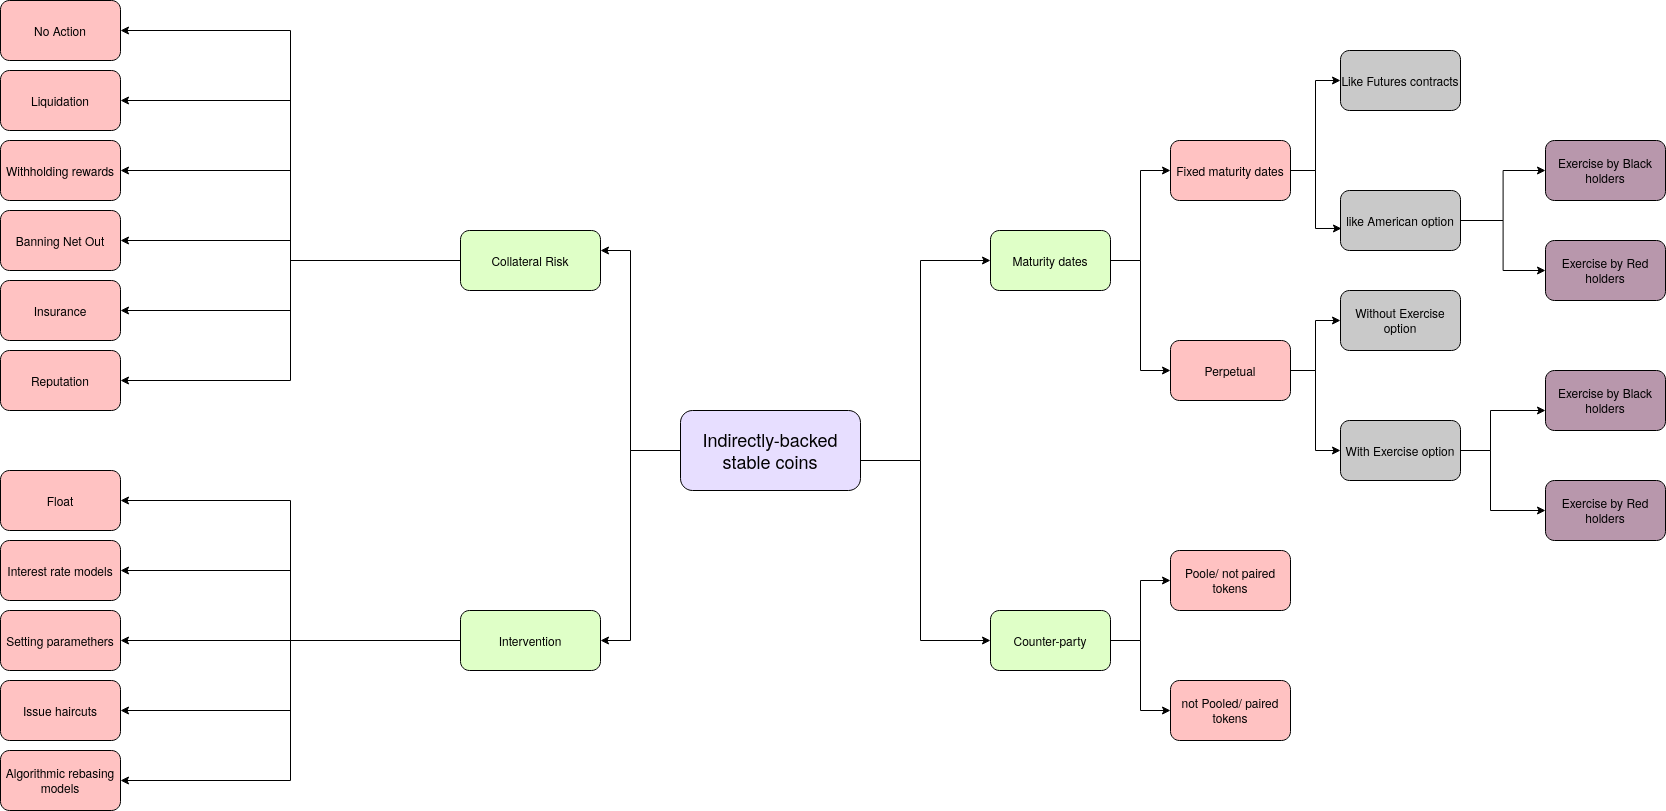
\includegraphics[width=12cm]{Mindmap}
\caption{overview of the indirectly-backed stablecoins design landscape}
\label{land}
\end{figure}

\subsection{Maturity Date}
The indirectly backed stable systems are agreements between two different parties, a stable party and a volatile party. These two parties should be different because holding both sides of the contract is equal to keeping the underlying asset on the wallet and it is not logical to participate on such a system to just keep the asset.

In this agreement the parties agree to split their deposited asset at a specified date named maturity date. At the maturity date the stable party will receive an exact amount of underlying asset based on the price of the asset at the settlement date and the volitile party will receive the remained part.

The first parameter that the designer should decide about is the maturity date. The maturity could be happened at a fixed specific time or could be perpetual.
\subsubsection{Fixed Maturity dates}
The designer can set specific dates for the contracts to be matured for example at the first day of each months. At the day of maturity the deposited assets are devided into two parts. The \$1 equivalent amount of the asset goes to the pocket of the stable party (if possible) and the remained is for volatile party. This is simlar to futures contract in Finance.

The designer may let one of the parties to exercise the contract beforr the maturity date. It is very similar to american options. The exerciser could be the black coin holder, red coin holder or both of them. 

\subsubsection{Perpetual contracts}
The other way to design the stable coin contracts is to make them as a perpetuty. In this mechanism there is no specific day for the parties to mature the contract. The system may have the option of settlement.

The perpetual stable coin without settlement is not rational because it is like burning the underlying asset to issue stable coins. 

For open-ended perpetual stable coins one of the parties has right to request for settlement whenever she wants. The exerciser could be black coin holder or red coin holder.
\subsection{Counter party}
One of the design parameters is to decide who is the risk taker in each contract. Each newly issued contract is backed by a different vault. Each black coin points its vault because the amount of deposits depend on the black coin holder decision. 
The designer could decide whether use a pool for red coins or pair each red coin to its related black coin.

\subsubsection{Pooled}

In this type of design the black coins are pointing to the vaults. Red coins are fungible on the system and there is no differences between them. There is no relations between red coin and the black coin. 

In this class, all red coin holders are risk takers of the system and on the unexpected events the take the risks regardless of their issuance contract.

In this case a black coin holder do not know the counterparty and the risk is pooled here.

\subsubsection{Paired}

The designer can create a system in which each red coin and black coins are paired and point to the issued contract. Now the black coin holders now their counterparty and the red coin holder is the risk taker of its own vault. So the risk is not pooled here.
\subsection{Collateral Risk}
If the price of the underlying asset goes down, the value of deposit falls below collateral ratio. The designers have the choice to react to this situation. We described some of different possible decisions:

\paragraph{Liquidation}
This variety of design is similar to the marginal accounts in traditional finance. If the underlying asset decreases in price and the value of a vault runs under the collateralization ratio, the system will liquidate the vault.

Liquidation occurs in the case that a vault is the danger area and may not able to pay its obligation. The deposited assets will transfer to the person who takes the responsibility of the debt of the vault. In other words, the liquidator should pay the borrowed red coin (and other obligations in a type of design, such as stability fee in MakerDAO) and receive the vault in exchange.


In liquidation design, the majority of vaults are over-collateralized. If a vault goes under-collateralize it will be liquidated. So, the red coin holders are pretty sure that their coin is backed by a dollar (. They can exchange their asset because the red coins are similar.

Smart contracts cannot trigger themselves. So, there should be an outsider player (like Keepers in MakerDao) to liquidate the warned vaults. They should trace the system to find the under-collateralized vaults and call the liquidation function. Then the keeper will transfer the debt of the vault to the smart contract and receive the deposit of the vault in exchange.

There are design parameters in the liquidation method:

\begin{enumerate}
  \item Collateralization Ratio:
This number shows the factor of over-collateralization. The ratio between the value of the deposits on each vault and the value of borrowed red coins should always be more than the collateralization ratio.
  
The collateralization ratio is depending on the volatility of the underlying asset. For instance, in the MakerDAO platform, the collateralization ratio for ETH vaults is 1.5. However, in the Synthetix project, it is 7.5 for SNX token, which is more volatile than ETH.
  \item Liquidation Incentive:
A smart contract is not able to trigger itself. An outsider player named liquidator should pay the transaction fee to call the liquidation function of the smart contract. Some factors influence the costs and profit of liquidators:
\begin{enumerate}
	\item Transaction fee:
The liquidator should trigger the liquidation function, send the sufficient red coins, and bid on the auction to win the vault. The user has to pay the transaction fee for these processes. The transaction fee depends on the time of transaction and network congestion.  
	\item Cost of capital: The liquidator pays the obligation by Red coin and receives the deposited coins of the vault. Therefore, the liquidator needs a sufficient amount of red coins for liquidation. There is an opportunity cost associated with the decision of the liquidator to not lend her capital and gain interest.

In other scenarios, the liquidator may just borrow the fund from lending platforms to liquidate the vault and pay back the loan afterward. There is a cost of borrowing in this scenario as well. So, there is a cost of capital for the liquidator.
	\item Price Oracles: RB coin systems need the price of the underlying asset in USD. Blockchains have no access to externals data. Oracles are outsider systems that collect the price and push them to the blockchains. Price inefficiency may impose extra costs on the liquidator. For instance, if the price of the asset is \$100 on the markets, although the oracle price is \$90, the liquidator spends more to provide liquidity from the markets.
\end{enumerate}  

The designer has to incentivize the liquidators to trace the blockchain, find alerted positions, and then send transactions to liquidate them. 

The mechanism of the incentivization is varied between protocols. A majority of platforms give the liquidator discounts on the vaults. For instance, in Single Collateral DAI (SAI), there was a \%3 discount on the liquidation process. Other platforms are using auction models to let the market decide about the value of the vault. 
  
  \item Auction model:
In the case of liquidations,  liquidators may come up with a specific warned position and want to liquidate it. The system designer has different options for the decision of picking the winner liquidator.
 
The simplest implementation mechanism is the First Come First Serve. However, it won't be fair for the vault holder if the first liquidator bids with a low amount of red coins.

There are other auction-based mechanisms to find the liquidator. The question raised here is, which method is the most efficient and fair auction model for both bidders and vault holders.

MakerDao utilizes a mixture of an absolute-auction and a reverse-auction model for the liquidation process.

The absolute auction model is used until the bids cover the debt of the vault. When the bids pass the debt, the auction reversed, the bidders bid on a lower amount of the deposits on the vault for a specific amount of DAI tokens, specified on the absolute auction step.
  
  \item Liquidation penalty:
The liquidation penalty is an extra punishment for the black coin holders to care about their debt to collateral ratio.
MakerDAO platform charges liquidated vault extra \%13 as a punishment for their vault holders. There are two main reasons to add Liquidation penalty on the design:

\begin{enumerate}

  \item To force vault keepers to be over-collateralized
  \item To mitigate grinding attacks: grinding attack occurs when the position holder deliberately unsafe her black coin and participate in the liquidation auction against her position to buy her deposited assets cheaper.

\end{enumerate}
\end{enumerate}

Using liquidation mechanism as a shield to protect the system provoke criticism. Possibly the black coin holders are freaking out when the price of ETH drops significantly. They may proceed to net out just before the liquidation occurs to their vaults. We called this situation "early liquidation" of the system. 

In this case, the system needs more ETHs to be deposited. The liquidation mechanism is designed to force the black coin holders to inject more ETHs to the system, but the black coin holders withdraw their deposits, and the total collateral of the system drops significantly, which is not the goal of the designers in this situation.

\paragraph{Withholding rewards}

Majority types of designs like liquidation are disincentivizing bad actors. But, another approach is to encourage users to act properly and incentivizing good actors of the system.

For instance, in the Synthetix project users need collateralize SNX tokens (Synthetix network token) to receive sUSD tokens (Synthetix stable coin pegging a USD). There is no margin call methods or liquidation function on the design. But, there is a reward on the system for users who keep more than the over-collateralization ratio. 
The Synthetix system has \%2 annual inflation on SNX tokens. The inflationary tokens are allocated to the vaults that hold more than the collateralization ratio.

There is another reward for the system. The traders on the exchange of the Synthetix project, pay transfer fees collected and distributed to the vaults holding more than the collateral ratio.

The system incentivizes people to stake their SNX token to be over-collateralized and receive the rewards. So, there is no punishment in the system for bad actors in this class of design.

\paragraph{Banning Black coin holders}

In the design of indirectly-backed stable coins, the red coins are not redeemable. In other words, the red coin holders cannot give back their red coins to receive \$1 of the deposited ETH in exchange. The red coin holder must own (or buy if possible) a black coin to net out a vault and receive the ETH.

In the liquidation scenario, the designer pushes black coin holders to be over-collateralized, applying liquidation punishments. Red coin holders and arbitragers are confident that there is no difference between the red coins because each of the red coins is backed by a sufficient amount of ETHs to be \$1 (with high probability).

In another class, the designer removes the liquidation mechanism, prevent black coin holders from withdrawal. In the fungible black coin design class, the designer also forbids the black coin holders from transferring their token. 

In this situation, the incentives for black coin holders to be over-collateralized has been decreased, compared to liquidation design class. But, there is a huge incentive left for them to be over-collateralized. If the price of the underlying asset drops, the black coin holders may want to sell their deposited assets to reduce the loss. In this scenario, just black coin holders that have over-collateralized vaults can net out and receive their underlying assets to sell them to the market.

This type of design will increase the fluctuation of the price of the red coin. The market watches the aggregated collaterals on the system and the number of red coins issued by the system and also the price of the underlying asset to evaluate the price of red coins. So when the price of underlying asset drops, the price of red coins will reduce concerning the underlying asset price. 

In this scenario, red coin holders are taking parts of the risk of underlying asset volatility risk. On the situation that the price of the asset drops significantly, the value of the stable coin will fall.

\paragraph{Reputation systems}

In traditional finance, reputation scoring systems are used to decrease or eliminate the collateral needs for a specific financial transaction. Participants are utilizing their reputation as collateral or source of trust for financial services. 

For instance, in the FICO credit score system, users can enhance their credit limit by increasing their credit score. There is a default risk on credit systems, but the defaulted person will be punished by credit score reduction. The bad actor loses reputation scores forbidden from using plenty of financial services. Therefore, users have adequate incentives to pay their bills.

A revolution of decentralizing the finance products on top of blockchain technologies began in early 2018, named Decentralized Finance (Defi) movement. There is a myriad of different decentralized financial services out there, such as MakerDAO, Compound, Synthetix, Aave, etc. 

There are no differences between users that act properly on Defi platforms and the bad actors. The DeFi ecosystem suffers from a lack of a reputation system or reputation scoring. Using a reputation system will incentivize users to act properly and also reduce the default risk of the system. On the other side of the coin, the users with high-grade reputation scores have new opportunities. So, the cost of defaulting will be increased for high-grade users.

There are barriers to implementing an effective reputation system on blockchains. Lack of strong identities or anonymity is one of them. Also, users can create fake histories. However, these are not impossible to address.

In case that our system concludes a trustworthy reputation system, the designer can use reputation as collateral.  We describe two different designs using reputation systems:
\begin{enumerate}
	\item Reputation-based collateral ratio: 
In the design of the system, the collateral ratio could be reliant on the reputation of the user. In other words, the collateral ratio is higher for new users (users with no reputation) and lower for users that act properly for a long time.
	\item Reputation-based staibility fee
In systems like MakerDAO, the DAI borrowers are obliged to pay a fee on their borrowing named stability fee. This stability fee is being set by Maker token holders.
	In a design based on the reputation, the stability fee could be dependent on the reputation of the user. The reputable user is paying a lower stability fee compared to the new users.
\end{enumerate}
 
\paragraph{Insurance}
Insurance models are used to hedge the risk of unexpected events in different systems. Under-collateralization of a vault is an unexpected event on the RBcoin system. The designer could use an insurance model to protect parties from financial loss in the case of under-collateralization. 

On the insurance model, the insurer will pay a premium to the insurance company. The company will protect the client from financial loss. 

In RBcoins there could be a built-in or outsourced insurance model to protect parties from under collateralization loss. The question raised here is who should pay the premium.

\begin{enumerate}
	\item Premium pay by Red coin holders:
It is very similar to Credit Default Swaps (CDS) on traditional finance. In this design, the approach is that the red coin holders are lending some amount of money to black coin holders. Therefore, black coin holders are borrowing from red coin holders to have a leveraged position on the underlying asset. In this situation, the red coin holders can pay an insurance premium to the contract to protect themselves from the default risk of black coin holders. In the case of under-collateralization, if the black coin holder cannot afford the loss, the insurance contract will pay the loss to the red coin holder.

This type of design is implemented on the MakerDAO platform. The DAI borrowers are paying a premium so-called stability fee to the system. These fees are collected on a pool named Maker Buffer pool. In the case of liquidation of a CDP, if the winner of the auction pays a lower amount of the obligation of the vault, the difference between the obligation and the paid amount will be paid by the Maker Buffer pool.

	\item Premium pay by Black coin holders
In this type of design, the black coin holders are paying the insurance premium. It is similar to regular insurance contracts in which the insurer buys an asset and guarantee it by paying a premium to insurance companies. For example, a person purchases a house and insure it.
Here the black coin holders are buying a position and pay the insurance premium. If the price of underlying asset drops and the vault going to be liquidated the insurance contract will pay on behalf of the insurer.
	\item Premium pay by both
In this scenario, both Red and Black coin holders are paying the insurance premium to ensure their positions. 
\end{enumerate}
\subsection{Intervention}

The designer should indicate the level of intervention on the system. There could be some mechanisms to change the level of properties on the system. For instance, the designer may use interest rate models, algorithmic models or secondary tokens to acheive a system property.

\subsubsection{Float}

The desiner may let the system to be free of human or algorithm intervenions. This is the most decentral type of design. This type of design benefits simlicity and decentrality but the red coins has fluctuations.

\subsubsection{Interest rate models}

Interest rates are tools that a system governer has to stimulate the demand or supply side of a system. The designer of indirectly-backed stable coins can use interest rate models on red coins or black coins (two different rates) to adjust the supply and demand of black coins and red coins in the system. This rates could be adjusted by human intervention like DAI or could be fully algorithmic.

\subsubsection{Parameter setting}

All types of the indirectly-backed stable coin system has some parameters in common such as collateral ratio. In specific designs, there are other design parameters added to the system such as maturity dates, insurance premium and rates. The designer may decide to intervene on the system and change these parameter over time. This intervention could be by humans or algorithmic. 

\subsubsection{Issue haircut}

The designer should indicate that in case that the price of underlying asset goes down, who is the risk taker of the system. On regular system risk taker of the system is black coin holders till the price falls strongly and the black coins worth zero, then the red coin holders take all the risk.

The designer has other option to divide the risk between red coin holders and black coin holders. The designer could set hair cut parameter a (< 1). It means that if the price of the underlying asset falls 1 percent the redcoin holder now takes a percent of the risk and the the black coin holder takes 1-a percent.

This haircut parameter could be changed during the time by human intervention or algorithmic.


\subsubsection{Algorithmic rebasing models}

The designer may use rebasing models to change the number of tokens in a way that at the end of each day the price of redcoins is exactly a dollar.
%
% ---- Bibliography ----
%
% BibTeX users should specify bibliography style 'splncs04'.
% References will then be sorted and formatted in the correct style.
%
% \bibliographystyle{splncs04}
% \bibliography{mybibliography}
%
\begin{thebibliography}{8}
\bibitem{ref_article1}
Author, F.: Article title. Journal \textbf{2}(5), 99--110 (2016)

\bibitem{ref_lncs1}
Author, F., Author, S.: Title of a proceedings paper. In: Editor,
F., Editor, S. (eds.) CONFERENCE 2016, LNCS, vol. 9999, pp. 1--13.
Springer, Heidelberg (2016). \doi{10.10007/1234567890}

\bibitem{ref_book1}
Author, F., Author, S., Author, T.: Book title. 2nd edn. Publisher,
Location (1999)

\bibitem{ref_proc1}
Author, A.-B.: Contribution title. In: 9th International Proceedings
on Proceedings, pp. 1--2. Publisher, Location (2010)

\bibitem{ref_url1}
LNCS Homepage, \url{http://www.springer.com/lncs}. Last accessed 4
Oct 2017
\end{thebibliography}
\end{document}
